\section*{BÀI TẬP CUỐI CHƯƠNG 6}
\subsection{Câu hỏi trắc nghiệm}
\Opensolutionfile{ans}[ans/ans-DCT9-9C6-BTCC]
\begin{ex}%[Dự án EX-9-Đề Cương Toán 9]%[Phan Minh Hue]%[9D4N1-1]
	Hàm số nào sau đây có dạng $y=ax^{2}$ $(a \neq 0)$?
\choice
{$y=\dfrac{3}{2x^{2}}$}
{$y=-3x$}
{\True $y=3x^{2}$}
{$y=\dfrac{3}{x^{2}}$}
	\loigiai{Hàm số có dạng $y=ax^{2}$ $(a \neq 0)$ là $y=3x^{2}$.}
\end{ex}
%%%====Câu 2
\begin{ex}%[Dự án EX-9-Đề Cương Toán 9]%[Phan Minh Hue]%[9D4N1-3]
	Đồ thị hàm số $y=ax^{2}$ $(a \neq 0)$ là một đường cong đi qua gốc tọa độ và nhận trục $Oy$ làm trục đối xứng. Đường cong đó được gọi là Parabol với đỉnh $O$. Khẳng định nào sau đây là \textbf{sai}?
	\choice
	{Đồ thị nhận trục tung làm trục đối xứng}
	{Với $a<0$ thì đồ thị nằm phía dưới trục hoành và $O(0;0)$ là điểm cao nhất của đồ thị}
	{\True Với $a>0$ thì đồ thị nằm phía trên trục hoành và $O(0;0)$ là điểm cao nhất của đồ thị}
	{Với $a>0$ thì đồ thị nằm phía trên trục hoành và $O(0;0)$ là điểm thấp nhất của đồ thị}
	\loigiai{Đồ thị của hàm số $y=ax^2$, $(a\neq 0)$ là một Parabol đi qua gốc tọa độ $O$, nhận $Oy$ là trục đối xứng ($O$ là đỉnh của Parabol).\\
		Nếu $a>0$ đồ thị nằm phía trên trục hoành và $O$ là điểm thấp nhất của đồ thị.\\
		Nếu $a<0$ đồ thị nằm phía dưới trục hoành và $O$ là điểm cao nhất của đồ thị.}
\end{ex}
\begin{ex}%[Dự án EX-9-Đề Cương Toán 9]%[Phan Minh Hue]%[9D4N1-3]
Điểm $M(-3;-9)$ thuộc đồ thị hàm số nào dưới đây?
	\choice
	{$y=\dfrac{-1}{3}x^{2}$}
	{$y=-x$}
	{\True$y=2x-3$}
	{$y=x^{2}+2$}
	\loigiai{Thay $x=-3$; $y=-9$ ta thấy $2\cdot(-3)-3=-9$.\\ Vậy điểm $M(-3;-9)$ thuộc đồ thị hàm số $y=2x-3$.}
\end{ex}
\begin{ex}%[Dự án EX-9-Đề Cương Toán 9]%[Phan Minh Hue]%[9D4H1-3]
Cho hàm số $y=f(x)=(2m+1)x^{2}$. Giá trị của $m$ để hàm số đi qua điểm $A(1;5)$.
	\choice
	{$m=1$}
	{$m=-1$}
	{$m=\dfrac{3}{2}$}
	{\True$m=2$}
	\loigiai{
		Thay tọa độ điểm $A(1;5)$ với $x=1$; $y=5$ vào hàm số ta được
	\begin{eqnarray*}
	(2m+1)1^{2}&=&5\\
	2m+1&=&5\\
	2m&=&4\\
	m&=&2
	\end{eqnarray*}
Vậy giá trị $m=2$ thì đồ thị của hàm số $y=f(x)=(2m+1)x^{2}$ đi qua $A(1;5)$.}
\end{ex}
\begin{ex}%[Dự án EX-9-Đề Cương Toán 9]%[Phan Minh Hue]%[9D4N1-3]
	Giá trị của hàm số $y=2x^{2}+1$ tại $x=-1$ là
	\choice
	{$3$}
	{$-1$}
	{\True$3$}
	{$0$}
	\loigiai{
		Thay $x=-2$ vào hàm số $y=f(x)=-7x^2$ ta được
	$y=2(-1)^{2}+10=2+1=3.$}
\end{ex}
\begin{ex}%[Dự án EX-9-Đề Cương Toán 9]%[Phan Minh Hue]%[9D4H1-3]
	\immini{
Hàm số nào dưới đây có đồ thị như hình bên
	\choice
	{$y=2x^{2}+1$}
	{$y=-x^{2}$}
	{\True$y=x^{2}$}
	{$y=3x$}}
{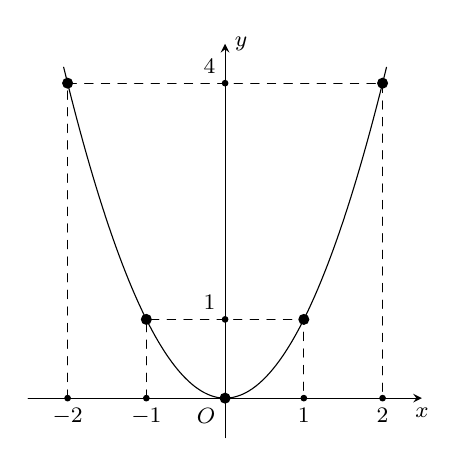
\begin{tikzpicture}[scale=1, font=\footnotesize, line cap=round, line join=round, >=stealth]
		\draw[->] (-2.5,0)--(2.5,0)node[below]{$x$};
		\draw[->] (0,-0.5)--(0,4.5)node[right]{$y$};
		\draw[domain=-2.05:2.05, samples=100] plot(\x,{(\x)^2});
		\draw[fill=black] (0,0)node[below left]{$O$}circle(1pt) (1,0)node[below]{$1$}circle(1pt) (0,4)node[above left]{$4$}circle(1pt) (0,1)node[above left]{$1$}circle(1pt) (2,0)node[below]{$2$}circle(1pt) (-2,0)node[below]{$-2$}circle(1pt) (-1,0)node[below]{$-1$}circle(1pt);
		\draw[dashed] (-1,0)--(-1,1)--(1,1)--(1,0)  (-2,0)--(-2,4)--(2,4)--(2,0);
		\fill (-1,1) circle (2pt) 	coordinate(A) ;
		\fill (1,1) circle (2pt) 	coordinate(B) ;
		\fill (2,4) circle (2pt) 	coordinate(C) ;
		\fill (-2,4) circle (2pt) 	coordinate(D) ;
		\fill (0,0) circle (2pt) 	coordinate(E) ;
\end{tikzpicture}}
\loigiai{Quan sát đồ thị ta thấy điểm $(1;1)$; $(-1;1)$; $(0;0)$; $(2;4)$ và $(-2;4)$ thuộc đồ thị hàm số. Thay giá trị vào các đáp án ta thấy đáp án thỏa mãn $5$ điểm là $y=x^{2}$.}
\end{ex}
\begin{ex}%[Dự án EX-9-Đề Cương Toán 9]%[Phan Minh Hue]%[9D4H1-3]
	Cho hàm số $y=ax^{2}$. Tìm hệ số $a$ biết đồ thị hàm số đi qua điểm $(2;4)$.
	\choice
	{\True$a=1$}
	{$a=2$}
	{$a=3$}
	{$a=-1$}
	\loigiai{Thay $x=2$; $y=4$ vào hàm số ta được $4=a\cdot2^{2}$.\\
	Do đó $a=1$.}
\end{ex}
\begin{ex}%[Dự án EX-9-Đề Cương Toán 9]%[Phan Minh Hue]%[9D4H1-3]
Cho hàm số $y=-2x^{2}$ có đồ thị Parabol $(P)$. Cho biết điểm $A(1;-2)$ thuộc đồ thị hàm số. Tính tổng khoảng cách từ điểm $A$ đến các trục tọa độ? 
	\choice
	{$4$}
	{$1$}
	{\True$3$}
	{$1$}
	\loigiai{Khoảng cách từ điểm $A(1;-2)$ đến trục hoành $Ox$ là $|x_A|=|1|=1$.\\
	Khoảng cách từ $A(1;-2)$ đến trục tung $Oy$ là $|y_A|=|-2|=2$.\\
	Tổng khoảng cách từ $A(1;-2)$ đến các trục tọa độ là $1+2=3$. }
\end{ex}
\begin{ex}%[Dự án EX-9-Đề Cương Toán 9]%[Phan Minh Hue]%[9D4N2-1]
	Phương trình nào sau đây là phương trình bậc hai một ẩn?
	\choice
	{$x-3=0$}
	{$0x^{2}+3x+1=0$}
	{\True $\sqrt{3} x^{2}-5=0$}
	{$\dfrac{3}{x^{2}}-2x=0$}
	\loigiai{Phương trình bậc hai một ẩn có dạng $ax^{2}+bx+c=0$ ($a\ne0$). \\Vậy $\sqrt{3} x^{2}-5=0$ là phương trình bậc hai một ẩn với $a=\sqrt3$; $b=0$ và $c=-5$.} 
\end{ex}
\begin{ex}%[Dự án EX-9-Đề Cương Toán 9]%[Phan Minh Hue]%[9D4H2-1]
		Cho phương trình $mx^{2}-4x-m=0$ (ẩn $x$, $m$ là tham số). Tìm điều kiện của $m$ để phương trình là phương trình bậc hai một ẩn.
	\choice
	{$m=0$}
	{\True$m\ne0$}
	{$m\ne4$}
	{$m\ne1$}
	\loigiai{Phương trình bậc hai $ax^{2}+bx+c=0$ là phương trình bậc hai một ẩn khi $a\ne0$. Do đó  $m\ne0$.} 
\end{ex}
\begin{ex}%[Dự án EX-9-Đề Cương Toán 9]%[Phan Minh Hue]%[9D4H2-1]
	Cho phương trình $(4-m^{2})x^3-(m+2)x^{2}+3x=0$ (ẩn $x$, $m$ là tham số). Tìm điều kiện của $m$ để phương trình là phương trình bậc hai một ẩn.
	\choice
	{$m\in\{-2;2\}$}
	{\True$m=2$}
	{$m=-2$}
	{$m\ne\{-2;2\}$}
	\loigiai{Điều kiện để phương trình là phương trình bậc hai một ẩn là
	$\heva{&4-m^{2}=0\\&m+2\ne0.}$\\
	Khi đó ta được 
	$\heva{&m=2\, \text{hoặc} \, m=-2\\&m\ne-2.}$\\
	Vậy $m=2$.}
\end{ex}
\begin{ex}%[Dự án EX-9-Đề Cương Toán 9]%[Phan Minh Hue]%[9D4H2-1]
Cho phương trình $2x^{2}-(m-1)x-2m-1=0$ ($x$ là ẩn, $m$ là tham số). Tìm giá trị của tham số $m$ để phương  trình có một nghiệm $x=-1$?
	\choice
	{$m=\dfrac{-1}{2}$}
	{$m=\dfrac{1}{2}$}
	{$m=1$}
	{\True$m=0$}
	\loigiai{
	Vì $x=-1$ là nghiệm của phương trình, nên ta có
	\begin{eqnarray*}
	2\cdot(-1)^{2}-(m-1)\cdot(-1)-2m-1&=&0\\
		2+m-1-2m-1&=&0\\
		-m&=&0\\
		m&=&0.
		\end{eqnarray*}}
\end{ex}
\begin{ex}%[Dự án EX-9-Đề Cương Toán 9]%[Phan Minh Hue]%[9D4N2-3]
	Phương trình $2x^{2}-4x+1=0$ có biệt thức $\Delta'$ bằng
	\choice
	{\True $2$}
	{$-2$}
	{$8$}
	{$6$}
	\loigiai{Ta có $a=2$; $b'=\dfrac{1}{2}\cdot b=-4$ và $c=1$.\\
		Phương trình $2x^{2}-4x+1=0$ có biệt thức $\Delta'=(-2)^{2}-2\cdot1=4-2=2$.
	}
\end{ex}
\begin{ex}%[Dự án EX-9-Đề Cương Toán 9]%[Phan Minh Hue]%[9D4N2-3]
	Hệ số $b'$ của phương trình $x^{2}+4(m-1)x+m=0$ có giá trị nào sau đây?
	\choice
	{$4(m-1)$}
	{$m$}
	{$(m-1)$}
	{\True $2(m-1)$}
	\loigiai{
	Phương trình $ax^{2}+bx+c=0$ có hệ số $b'=\dfrac{1}{2}\cdot b$.\\
	Phương trình $x^{2}+4(m-1)x+m=0$ có giá trị $b=4(m-1)$ nên $b'=2(m-1)$.
	}
\end{ex}
\begin{ex}%[Dự án EX-9-Đề Cương Toán 9]%[Phan Minh Hue]%[9D4N2-1]
	$x=2$ là nghiệm của phương trình nào dưới đây?
	\choice
	{$x^{2}+x+1=0$}
	{$x^{2}-3x+2=x$}
	{$x^4-4=0$}
	{\True $-x^{2}+x+2=0$}
	\loigiai{
		Thay $x=2$ vào lần lượt từng phương trình. Tại phương trình nào khi thay $x=2$ cho kết quả hai vế bằng nhau thì kết luận $x=2$ là nghiệm của phương trình.
		\begin{itemize}
			\item $x^{2}+x+1=0$ (1). Thay $x=2$ vào phương trình (1) ta được $2^{2}+1\cdot2+1=7$.\\
			Vậy $x=2$ không là nghiệm của phương trình.
			\item $2x^{2}-3x=x$ (2). Thay $x=2$ vào phương trình (2)
			ta có $VT=2^{2}-3\cdot2=-2$.\\
			Suy ra $VT\neq VP$ $(VP=2)$.\\
			Vậy $x=2$ không là nghiệm của phương trình.
			\item $x^4-1=0$ (3) thay $x=2$ vào phương trình (3) ta được $2^4-1=15$.\\
			Vậy $x=2$ không là nghiệm của phương trình.
			\item $x^{2}-2x=0$ (4). Thay $x=2$ vào phương trình (4) ta được $2^{2}-2\cdot2=0$.\\
			Vậy $x=2$ là nghiệm của phương trình.
		\end{itemize}}
\end{ex}
\begin{ex}%[Dự án EX-9-Đề Cương Toán 9]%[Phan Minh Hue]%[9D4N2-3]
	Cho phương trình bậc hai $ax^{2}+bx+c=0$ $(a\neq0)$. Nếu $b^{2}-4ac>0$ thì phương trình có hai nghiệm phân biệt là
	\choice
	{$x_1=\dfrac{-b-\sqrt{\Delta}}{a}$; $x_2=\dfrac{-b+\sqrt{\Delta}}{a}$}
	{\True $x_1=\dfrac{-\sqrt{\Delta}-b}{2a}$; $x_2=\dfrac{\sqrt{\Delta}-b}{2a}$}
	{$x_1=\dfrac{b-\sqrt{\Delta}}{2a}$; $x_2=\dfrac{b+\sqrt{\Delta}}{2a}$}
	{$x_1=\dfrac{b+\sqrt{\Delta}}{2a}$; $x_2=\dfrac{-b+\sqrt{\Delta}}{2a}$}
	\loigiai{
	Phương trình có $b^{2}-4ac>0$ thì phương trình có hai nghiệm phân biệt là $x_1=\dfrac{-\sqrt{\Delta}-b}{2a}$; $x_2=\dfrac{\sqrt{\Delta}-b}{2a}$.}
\end{ex}
\begin{ex}%[Dự án EX-9-Đề Cương Toán 9]%[Phan Minh Hue]%[9D4N2-3]
	Cho phương trình bậc hai $ax^{2}+bx+c=0$ $(a\neq0)$. Nếu $b^{2}-4ac=0$ thì phương trình có nghiệm kép là
	\choice
	{$x_1=x_2=-\dfrac{a}{2b}$}
	{$x_1=x_2=-\dfrac{b}{a}$}
	{$x_1=x_2=-\dfrac{c}{a}$}
	{\True $x_1=x_2=-\dfrac{1}{2}\cdot\dfrac{b}{a}$}
	\loigiai{
	Phương trình có $\Delta=0$ thì phương trình có nghiệm kép $x_1=x_2=-\dfrac{b}{2a}$ .}
\end{ex}
\begin{ex}%[Dự án EX-9-Đề Cương Toán 9]%[Phan Minh Hue]%[9D4N3-1]
	Phương trình $ax^2+bx+c=0$ $(a\neq0)$ có $a+b+c=0$. Khi đó
	\choice
	{\True Phương trình có một nghiệm $x_1=1$, nghiệm kia là $x_2=\dfrac{c}{a}$}
	{Phương trình có một nghiệm $x_1=-1$, nghiệm kia là $x_2=\dfrac{c}{a}$}
	{Phương trình có một nghiệm $x_1=-1$, nghiệm kia là $x_2=-\dfrac{c}{a}$}
	{Phương trình có một nghiệm $x_1=1$, nghiệm kia là $x_2=-\dfrac{c}{a}$}
	\loigiai{
		\begin{itemize}
			\item Nếu phương trình $ax^2+bx+c=0$ $(a\neq0)$ có $a+b+c=0$ thì phương trình có một nghiệm là $x_1=1$, còn nghiệm kia là $x_2=\dfrac{c}{a}$.
			\item Nếu phương trình $ax^2+bx+c=0$ $(a\neq0)$ có $a-b+c=0$ thì phương trình có một nghiệm là $x_1=-1$, còn nghiệm kia là $x_2=-\dfrac{c}{a}$.
		\end{itemize}
	}
\end{ex}
\begin{ex}%[Dự án EX-9-Đề Cương Toán 9]%[Phan Minh Hue]%[9D4H2-3]
	Với giá trị nào của $m$ thì phương trình bậc hai $x^{2}-2mx+1=0$ có nghiệm kép
	\choice
	{$m=1$}
	{$m=-1$}
	{\True $m=1$ hoặc $m=-1$}
	{$m=2$}
	\loigiai{Ta có $a=1$; $b=-2m$; $c=1$. Do đó $\Delta=4m^{2}-4$.\\
	Phương trình $x^{2}-mx+1=0$ có nghiệm kép thì $\Delta=0$. Suy ra $m=\pm1$.
	}
\end{ex}
\begin{ex}%[Dự án EX-9-Đề Cương Toán 9]%[Phan Minh Hue]%[9D4H2-2]
Hệ số $a$, $b$, $c$ của phương trình bậc hai $2x^2-3x+1=0$ là
	\choice
{\True $a=2$, $b=-3$, $c=1$}
{$a=2$, $b=3$, $c=1$}
{$a=2$, $b=-3$, $c=-1$}
{$a=1$, $b=-3$, $c=1$}
\loigiai{Phương trình có $a=2$, $b=-3$, $c=1$.}
\end{ex}
\begin{ex}%[Dự án EX-9-Đề Cương Toán 9]%[Phan Minh Hue]%[9D4H2-2]
	Cho hai hàm số sau $y=x^{2}$ và $y=2x-1$. Xác định tọa độ giao điểm của hai đồ thị hàm số trên.
	\choice
	{\True$M(1;1)$}
	{$M(1;1)$ và $N(-1;1)$}
	{$N(-1;1)$}
	{$N(1;2)$}
	\loigiai{
		Hoành độ giao điểm hai đồ thị là nghiệm của phương trình 
		\begin{eqnarray*}
			x^{2}&=&2x-1\\
			x^{2}-2x+1&=&0\\
			(x-1)^{2}&=&0\\
			x-1&=&0\\
			x&=&1.
		\end{eqnarray*}
		Với $x=1$ ta có $y=1$. Vậy giao điểm đồ thị hai hàm số là $M(1;1)$.}
\end{ex}
\begin{ex}%[Dự án EX-9-Đề Cương Toán 9]%[Phan Minh Hue]%[9D4N2-3]
	Phương trình $-x^{2}+4x+5=0$ có một nghiệm là
	\choice
	{$x=4$}
	{\True $x=-1$}
	{$x=-5$}
	{$x=1$}
	\loigiai{
	Ta có $a=-1$; $b=4$; $c=5$. Vì $a-b+c=-1-4+5=0$ nên phương trình có một nghiệm là $x=-1$.
	}
\end{ex}
\begin{ex}%[Dự án EX-9-Đề Cương Toán 9]%[Phan Minh Hue]%[9D4N2-3]
	Phương trình bậc hai $2x^{2}-kx-10=0$ có một nghiệm là $5$. Tìm nghiệm  còn lại của phương trình.
	\choice
	{$x=1$}
	{$x=2$}
	{$x=-2$}
	{\True$x=-1$}
	\loigiai{Thay $x=5$ vào phương trình ta có
			\begin{eqnarray*}
			2\cdot5^2-k\cdot5-10&=&0\\
			50-5k-10&=&0\\
		40&=&5k\\
			k&=&8.
		\end{eqnarray*} 
		Phương trình có hai nghiệm, theo định lý Viète ta có 
		$\heva{&x_1+x_2=\dfrac{k}{2}=\dfrac{8}{2}=4\\&x_1\cdot x_2=-5.}$\\
	Vì $x_1=5$ do đó $5+x_2=4$.
	Vậy $x_2=-1$.}	
\end{ex}
\begin{ex}%[Dự án EX-9-Đề Cương Toán 9]%[Phan Minh Hue]%[9D4N2-3]
	Cho phương trình bậc hai $x^{2}-8x-1=0$. Tính $x_1+x_2$.
	\choice
	{$\dfrac{1}{8}$}
	{\True $8$}
	{$-8$}
	{$-1$}
	\loigiai{Ta có $a=1$; $b=-8$; $c=-1$.\\
		Theo định lý Viète ta có $x_1+x_2=-\dfrac{b}{a}=-\dfrac{-8}{1}=8$.}
\end{ex}
\begin{ex}%[Dự án EX-9-Đề Cương Toán 9]%[Phan Minh Hue]%[9D4N3-2]
	Biết $u+v=3$, $u\cdot v=-4$ và $u > v$. Khi đó, hiệu $u-v$ bằng
	\choice
	{$3$}
	{$-4$}
	{\True $5$}
	{$-5$}
	\loigiai{
		Vì $u+v=3$ và $u\cdot v=-4$ nên $u$ và $v$ là hai nghiệm của phương trình $x^{2}-3x-4=0$.\\
		Ta có $a=1$; $b=-3$; $c=-4$ khi đó $\Delta=b^2-4ac=9-4\cdot1\cdot(-4)=25$.\\ Vì $\Delta>0$ nên phương trình có hai nghiệm phân biệt\\ $x_1=\dfrac{-b-\sqrt{\Delta}}{2a}=\dfrac{3-\sqrt25}{2}=-1$; $x_1=\dfrac{-b+\sqrt{\Delta}}{2a}=\dfrac{3+\sqrt25}{2}=4$.\\
		Lại có $u>v$ nên $u=4$ và $v=-1$.\\
		Vậy $u-v=4-(-1)=5$.
	}
\end{ex}

\begin{ex}%[Dự án EX-9-Đề Cương Toán 9]%[Phan Minh Hue]%[9D4N3-1]
Gọi $x_1$, $x_2$ là hai nghiệm của phương trình bậc hai $-x^{2}-7x+12=0$. Khi đó giá trị của biểu thức $7(x_1+x_2)-4x_1x_2$ bằng
	\choice
	{\True$1$}
	{$-1$}
	{\True $-97$}
	{$97$}
	\loigiai{Ta có $a=-1$; $b=-7$; $c=12$.\\
		Vì $x_1;x_2$ là hai nghiệm của phương trình. Áp dụng định lý Viète  ta có
			$\heva{&x_1+x_2=-7\\&x_1\cdot x_2=-12.}$\\
	Ta có $7(x_1+x_2)-4x_1x_2=7\cdot(-7)-4\cdot(-12)=-1$.
	}
\end{ex}
\begin{ex}%[Dự án EX-9-Đề Cương Toán 9]%[Phan Minh Hue]%[9D4V2-3]
	Một quả bóng được ném lên theo phương thẳng đứng từ mặt đất với vận tốc ban đầu là $9{,}8$ m/s. Khi bỏ qua sức cản của không khí, độ cao $h$ (m) của quả bóng so với mặt đất được tính theo thời gian $t$ (giây) bởi công thức $h(t)=-4{,}9t^{2}+9{,}8t+40$ $(t \geq 0)$. Trong thời điểm nào thì quả bóng ở độ cao $0{,}8$ m.
	\choice
	{$4$ (giây)}
	{$2$ (giây)}
	{\True $3$ (giây)}
	{$5$ (giây)}
	\loigiai{
		Khi quả bóng ở độ cao $0{,}8$ m ta có $-4{,}9t^{2}+9{,}8t+40=0{,}8$.\\
		Khi đó $-4{,}9t^{2}+9{,}8t+39{,}2=0$.\\
		$\Delta=b^2-4ac=(9{,}8)^2-4\cdot-4{,}9\cdot39{,}2=864{,}36$.\\
		Vì $\Delta>0$ nên phương trình có hai nghiệm phân biệt\\ $x_1=\dfrac{-b-\sqrt{\Delta}}{2a}=\dfrac{-9{,}8-\sqrt{864,36}}{2\cdot-4{,}9}=4$ (thỏa mãn điều kiện);\\ 
		$x_1=\dfrac{-b-\sqrt{\Delta}}{2a}=\dfrac{-9{,}8+\sqrt{864,36}}{2\cdot-4{,}9}=-2$ (không thỏa mãn điều kiện).\\
		Vậy sau $4$ giây, quả bóng ở độ cao $0{,}8$ m.
	}
\end{ex}
\begin{ex}%[Dự án EX-9-Đề Cương Toán 9]%[Phan Minh Hue]%[9D4V3-1]
	Cho phương trình bậc hai $x^{2}-2x-m^{2}=0$. Tìm giá trị của $m$ để phương trình có hai nghiệm phân biệt $x_1$, $x_2$ thỏa mãn $(x_1+1)(x_2+1)=-3$.
	\choice
	{\True$m=-\sqrt6$; $m=-\sqrt6$}
	{$m=6$}
	{$m=2$; $m=-2$}
	{$m=\sqrt6$}
	\loigiai{
	Ta có $a=1$; $b=-2$; $c=-m^2$; $\Delta=b^2-4ac=(-2)^2-4\cdot1\cdot(-m)^2=4+4m^2$.\\
	Vì $m^2\geq0$ với mọi giá trị của $m$ nên $4+4m^2>0$ với mọi giá trị của $m$.\\ Do đó phương trình luôn có hai nghiệm phân biệt. Gọi $x_1$; $x_2$ là hai nghiệm của phương trình.\\
	Áp dụng định lý Viète  ta có 	$\heva{&x_1+x_2=2\\&x_1\cdot x_2=-m^{2}.}$\\
	Ta có 	\begin{eqnarray*}
	(x_1+1)(x_2+1)&=&-3\\
		x_1+x_2+x_1x_2+4&=&0\\
		2-m^{2}+4&=&0\\
		m&=&\pm\sqrt6.
	\end{eqnarray*}
	}
\end{ex}
\begin{ex}%[Dự án EX-9-Đề Cương Toán 9]%[Phan Minh Hue]%[9D4N2-5]
Một phân xưởng theo kế hoạch cần sản xuất $140$ sản phẩm trong thời gian quy định. Do mỗi ngày phân xưởng vượt mức $2$ sản phẩn nên đã hoàn thành sớm hơn dự định $2$ ngày. Tìm phương trình biểu diễn bài toán biết số sản phẩm mỗi ngày  theo kế hoạch của phân xưởng là $x$.
	\choice
	{\True$\dfrac{140}{x}-\dfrac{140}{x+2}=2$}
	{$\dfrac{140}{x}-\dfrac{140+2}{x}=2$}
	{$\dfrac{140}{x+2}-\dfrac{140}{x}=2$}
	{$\dfrac{140}{x}=\dfrac{140+2}{x+2}$}
	\loigiai{
Số sản phẩm mỗi ngày thực tế làm là $x+2$ (sản phẩm).\\
Thời gian hoàn thành theo kế hoạch là $\dfrac{140}{x}$ (ngày).\\
Thời gian hoàn thành thực tế là $\dfrac{140}{x+2}$ (ngày).\\
Vì thực tế hoàn thành sớm hơn dự định $2$ ngày nên ta có phương trình 
$$\dfrac{140}{x}-\dfrac{140}{x+2}=2.$$
}
\end{ex}
\begin{ex}%[Dự án EX-9-Đề Cương Toán 9]%[Phan Minh Hue]%[9D4H2-5]
	Một ca nô chạy ngược dòng trên quãng sông $AB$ dài $72$ km. Biết vận tốc dòng nước là $2$ km/h và vận tốc thực của ca nô là $x$ km/h $(x>2)$. Thời gian ca nô đi ngược dòng hết quãng đường $AB$ là 
	\choice
	{$x-2$}
	{$x+2$}
	{$\dfrac{72}{x+2}$}
	{\True$\dfrac{72}{x-2}$}
	\loigiai{
Vận tốc ca nô ngược dòng là $x-2$ $(\text{km/h})$.\\
Thời gian ca nô ngược dòng là $\dfrac{72}{x-2}$ (giờ).}
\end{ex}
\Closesolutionfile{ans}
\begin{indapan}{5}
	{ans/ans-DCT9-9C6-BTCC}
\end{indapan}
\subsection{Bài tập tự luận}
\begin{bt}%[Dự án EX-9-Đề Cương Toán 9]%[Phan Minh Hue]%[9D4N1-2]
	Cho hàm số $y=2x^{2}$. Tìm giá trị của $y$ tương ứng với giá trị của $x$ trong bảng như sau
	\begin{center}
		\begin{tabular}{|c|c|c|c|c|c|c|c|}
			\hline
			$x$ & $-2$ & $-1$ & $0$ & $1$ & $2$ \\
			\hline
			$y=2x^{2}$ & & & & & \\
			\hline
		\end{tabular}
	\end{center}
	\loigiai{
		Để tìm giá trị của $y$ tương ứng với mỗi giá trị của $x$, ta thay giá trị của $x$ vào hàm số $y=2x^{2}$ và tính toán.
		\begin{center}
			\begin{tabular}{|c|c|c|c|c|c|c|c|}
				\hline
				$x$ & $-2$ & $-1$ & $0$ & $1$ & $2$ \\
				\hline
				$y=2x^{2}$ & $8$ & $2$ & $0$ & $2$ & $8$ \\
				\hline
			\end{tabular}
		\end{center}
	}
\end{bt}
\begin{bt}%[Dự án EX-9-Đề Cương Toán 9]%[Phan Minh Hue]%[9D4V1-1]
	Cho hàm số $y=f(x)=\dfrac{3}{5}x^{2}$.
		\begin{enumerate}
		\item  Tính $f(-2)+f(1)$.
		\item Tìm các giá trị của nguyên dương của $m$ để $f(m+1)=15$.
	\end{enumerate}
	\loigiai{
		\begin{enumerate}
		\item Ta có $f(-2)+f(1)=\dfrac{3}{5}\cdot(-2)^{2}+\dfrac{3}{5}\cdot1^{2}=\dfrac{3}{5}\cdot 4+\dfrac{3}{5}\cdot 1=\dfrac{12}{5}+\dfrac{3}{5}=\dfrac{15}{5}=3.$\\
		Vậy $f(-2)+f(1)=3$.
		\item Ta có 
		\begin{eqnarray*}
				f(m+1)&=&15\\
				\dfrac{3}{5}(m+1)^{2}&=&15\\
			(m+1)^{2}&=&\dfrac{75}{3}\\
			(m+1)^{2}&=&25.
		\end{eqnarray*}
	Trường hợp 1 
	\begin{eqnarray*}
		m+1&=&5\\
		m&=&4.
	\end{eqnarray*}
	Trương hợp 2
	\begin{eqnarray*}
		m+1&=&-5\\
		m&=&-6.
	\end{eqnarray*}
Vì $m$ là số nguyên dương. Vậy $m=4$.
	\end{enumerate}
	}
		\end{bt}

\begin{bt}%[Dự án EX-9-Đề Cương Toán 9]%[Phan Minh Hue]%[9D4H1-3]
	Cho hàm số $y=ax^{2}$ có đồ thị là parabol $(P)$. Điểm $M(2;-1)$ thuộc đồ thị hàm số trên.
		\begin{enumerate}
		\item Tìm hệ số $a$.
		\item Với hệ số $a$ vừa tìm được. Điểm $A(4;-4)$ có thuộc đồ thị hàm số không?
		\item Với hệ số $a$ vừa tìm được. Tìm các điểm trên $(P)$ có tung độ bằng $-4$.
	\end{enumerate}
	\loigiai{
		\begin{enumerate}
			\item Vì $M(2;-1)$ thuộc đồ thị hàm số nên ta thay $x=2$; $y=-1$ vào hàm số.\\
			Ta có	$-1=a\cdot2^{2}$.\\
			Do đó $a=-\dfrac{1}{4}$.
		     \item Với $a=-\dfrac{1}{4}$ hàm số có dạng $y=-\dfrac{1}{4}x^{2}$. Thay tọa độ điểm $A$ với $x=4;y=-4$, ta có
		     $$-\dfrac{1}{4}\cdot4^{2}=-\dfrac{1}{4}\cdot16=-4.$$
		     Vậy $A(4;-4)$ có thuộc đồ thị hàm số.
		     \item Gọi $M(x_M;y_M)$ là điểm thuộc đồ thị (P). Thay $y_M=-4$ vào hàm số, ta có
		     \begin{eqnarray*}
		     	-\dfrac{1}{4}\cdot x_M^{2}&=&-4\\
		     	x_M^{2}&=&16
		     \end{eqnarray*}
		     Do đó $x_M=4$ hoặc $x_M=-4$.
		     Vậy các điểm trên $(P)$ có tung độ là $-4$ là $(4;-4)$ và $(-4;-4)$.
		\end{enumerate}
	}
\end{bt}
\begin{bt}%[Dự án EX-9-Đề Cương Toán 9]%[Phan Minh Hue]%[9D4H1-3]
Vẽ đồ thị các hàm số sau
	\begin{multicols}{2}
	\begin{enumerate}
\item $y=x^2$;
\item $y=-\dfrac{3}{2}x^{2}.$
\end{enumerate}
	\end{multicols}
\loigiai{
	\begin{enumerate}
		\item 	Bảng giá trị
		\begin{center}
			\begin{tabular}{|c|c|c|c|c|c|}
				\hline
				$x$ & $-2$ & $-1$ & $0$ & $1$ & $2$\\
				\hline
				$y=x^2$ & $4$ & $1$ & $0$ & $1$ & $4$\\
				\hline
			\end{tabular}
		\end{center}
		Đồ thị hàm số là đường cong đi qua $5$ điểm $(-2;4)$; $(-1;1)$; $(0;0)$; $(1;1)$ và $(2;4)$.
		\begin{center}
			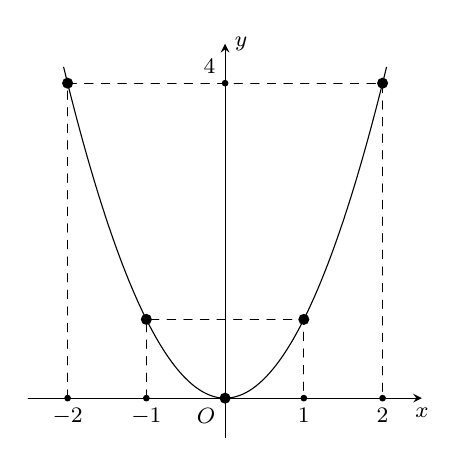
\begin{tikzpicture}[scale=1, font=\footnotesize, line cap=round, line join=round, >=stealth]
				\draw[->] (-2.5,0)--(2.5,0)node[below]{$x$};
				\draw[->] (0,-.5)--(0,4.5)node[right]{$y$};
				\draw[domain=-2.05:2.05, samples=100] plot(\x,{(\x)^2});
				\draw[fill=black] (0,0)node[below left]{$O$}circle(1pt) (1,0)node[below]{$1$}circle(1pt) (0,4)node[above left]{$4$}circle(1pt) (2,0)node[below]{$2$}circle(1pt) (-2,0)node[below]{$-2$}circle(1pt) (-1,0)node[below]{$-1$}circle(1pt);
				\draw[dashed] (-1,0)--(-1,1)--(1,1)--(1,0)  (-2,0)--(-2,4)--(2,4)--(2,0);
					\fill (-1,1) circle (2pt) 	coordinate(A) ;
				\fill (1,1) circle (2pt) 	coordinate(B) ;
				\fill (2,4) circle (2pt) 	coordinate(C) ;
				\fill (-2,4) circle (2pt) 	coordinate(D) ;
					\fill (0,0) circle (2pt) 	coordinate(E) ;
			\end{tikzpicture}
		\end{center}
	\item	Bảng giá trị
	\begin{center}
		\begin{tabular}{|c|c|c|c|c|c|}
			\hline
			$x$ & $-2$ & $-1$ & $0$ & $1$ & $2$\\
			\hline
			$y=-\dfrac{3}{2}x^{2}$ & $-6$ & $-1{,}5$ & $0$ & $-1{,}5$ & $-6$\\
			\hline
		\end{tabular}
	\end{center}
	Đồ thị hàm số là đường cong đi qua $5$ điểm $(-2;6)$; $(-1;-1,5)$; $(0;0)$; $(1;-1,5)$ và $(2;-6)$.
	\begin{center}
		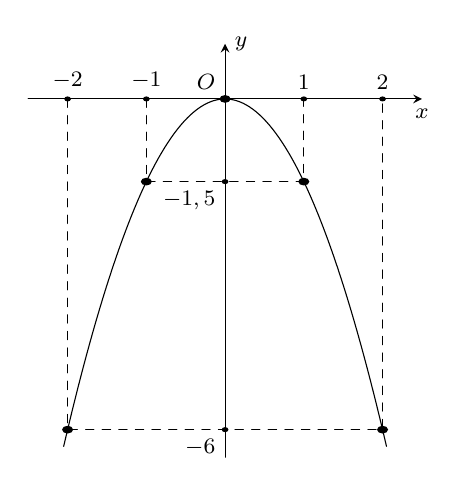
\begin{tikzpicture}[scale=1, yscale=0.7, font=\footnotesize, line cap=round, line join=round, >=stealth]
			\draw[->] (-2.5,0)--(2.5,0)node[below]{$x$};
			\draw[->] (0,-6.5)--(0,1)node[right]{$y$};
			\draw[domain=-2.05:2.05, samples=100] plot(\x,{-1.5*(\x)^2});
			\draw[fill=black] (0,0)node[above left]{$O$}circle(1pt) (1,0)node[above]{$1$}circle(1pt) (0,-1.5)node[below left]{$-1,5$}circle(1pt) (0,-6)node[below left]{$-6$}circle(1pt) (2,0)node[above]{$2$}circle(1pt) (-2,0)node[above]{$-2$}circle(1pt)
			 (-1,0)node[above]{$-1$}circle(1pt);
			\draw[dashed] (-1,0)--(-1,-1.5)--(1,-1.5)--(1,0)  (-2,0)--(-2,-6)--(2,-6)--(2,0);
				\fill (-1,-1.5) circle (2pt) 	coordinate(A) ;
			\fill (1,-1.5) circle (2pt) 	coordinate(B) ;
			\fill (-2,-6) circle (2pt) 	coordinate(C) ;
			\fill (2,-6) circle (2pt) 	coordinate(D) ;
			\fill (0,0) circle (2pt) 	coordinate(E) ;
		\end{tikzpicture}
	\end{center}
\end{enumerate}}
\end{bt}
\begin{bt}%[Dự án EX-9-Đề Cương Toán 9]%[Phan Minh Hue]%[9D4H2-1]
Phương trình nào dưới đây \textbf{không} là phương trình bậc hai một ẩn?
	\begin{multicols}{3}
	\begin{enumerate}
		\item $3x+2y=1$;
		\item $x^{2}-3x=5$;
		\item $x^{2}-6x+5=x(x+1)$;
		\item $y^{2}+y^{3}=2$;
		\item $3-x^{2}=1$;
		\item $x^{2}=6$;
	\end{enumerate}
\end{multicols}
	\loigiai{
\begin{enumerate}
	\item $3x+2y=1$ không phương trình bậc hai một ẩn;
	\item $x^2-3x=5$ là phương trình bậc hai một ẩn với $a=1$; $b=-3$; $c=-5$;
	\item \begin{eqnarray*}
		x^{2}-6x+5&=&x(x+1)\\
		x^{2}-6x+5&=&x^{2}+x\\
		-7x+5&=&0.
	\end{eqnarray*}
	Đây không phải là phương trình bậc hai một ẩn vì $a=0$.
\item $y^{2}+y^{3}=2$ không phải phương trình bậc hai một ẩn;
\item $3-x^2=1$ hay $-x^2+2=0$ là phương trình bậc hai một ẩn với $a=-1$; $b=0$; $c=2$;
\item $x^2=6$ là phương trình bậc hai một ẩn với $a=1$; $b=0$; $c=-6$;
\end{enumerate}}
\end{bt}
\begin{bt}%[Dự án EX-9-Đề Cương Toán 9]%[Phan Minh Hue]%[9D4H2-1]
	Trong các phương trình sau, những phương trình nào là phương trình bậc hai ẩn $x$? Chỉ rõ các hệ số $a$, $b$, $c$ của phương trình đó.
\begin{multicols}{2}
	\begin{enumerate}
		\item $x^{2}+\sqrt5x+1=0$;
		\item $\left(\dfrac{1}{x}\right)^{2}-\left(\dfrac{1}{x}\right)=0$;
		\item $-x^{2}=0$.
		\item $-x^{3}+2x^{2}=5$.
	\end{enumerate}
\end{multicols}
\loigiai{
	\begin{enumerate}
		\item Phương trình $x^{2}+\sqrt5x+1=0$ là phương trình bậc hai ẩn $x$ với $a=1$; $b=\sqrt5$; $c=1$;
		\item Phương trình $\left(\dfrac{1}{x}\right)^{2}-\left(\dfrac{1}{x}\right)=0$ không là phương trình bậc hai ẩn $x$;
		\item $-x^{2}=0$ là phương trình bậc hai ẩn $x$ với $a=-1$; $b=0$; $c=0$;
		\item Phương trình $-x^{3}+2x^{2}=5$ không là phương trình bậc hai ẩn $x$.
	\end{enumerate}
}
\end{bt}
\begin{bt}%[Dự án EX-9-Đề Cương Toán 9]%[Phan Minh Hue]%[9D4H2-3]
	Viết lại các phương trình sau dưới dạng $ax^{2}+bx+c=0, (a\ne0)$ và xác định các hệ số $a$, $b$, $c$ của từng phương trình.
	\begin{enumerate}
		\item $3x^{2}-5x+1=2x-3$;
		\item $\sqrt{2}x^{2}+3x-\sqrt{5}-x^{2}=0$;
		\item $mx^{2}-x=x^{2}+2mx-5m+1$;
		\item $m^{2}x+n\cdot x=2mn\cdot x^{2}-2$ (trong đó $m$, $n$ là các tham số).
	\end{enumerate}
\loigiai{
	\begin{enumerate}
		\item Ta có
		\begin{eqnarray*}
			3x^{2}-5x+1&=&2x-3\\
			3x^{2}-7x+4&=&0.
		\end{eqnarray*}
		Hệ số $a=3$; $b=-7$; $c=4$.
		\item Ta có
		\begin{eqnarray*}
			3x^{2}-5x+1&=&2x-3\\
			3x^{2}-7x+4&=&0.
		\end{eqnarray*}
		Hệ số $a=3$; $b=-7$; $c=4$.
		\item Ta có
		\begin{eqnarray*}
			mx^{2}-x&=&x^{2}+2mx-5m+1\\
			(m-1)x^{2}-(1+2m)x+5m-1&=&0.
		\end{eqnarray*}
		Hệ số $a=m-1$; $b=-1-2m$; $c=5m-1$.
		\item Ta có
		\begin{eqnarray*}
			m^{2}x+n\cdot x&=&2mn\cdot x^{2}-2\\
			2mnx^{2}-\left(m^{2}+n\right)x-2&=&0.
		\end{eqnarray*}
		Hệ số $a=2mn$; $b=-m^{2}-n$; $c=-2$.
	\end{enumerate}
}
\end{bt}
\begin{bt}%[Dự án EX-9-Đề Cương Toán 9]%[Phan Minh Hue]%[9D4H2-3]
Tìm giá trị của tham số $m$ để các phương sau là phương trình bậc hai một ẩn?
		\begin{enumerate}
			\item $mx^{2}-4x=3$;
			\item $(1-3m)x^{2}-2x+5=0$;
			\item $(m^{2}-1)x^{2}+(m+1)x=0$;
			\item $mx^{3}+(m+1)x^{2}-5=0$;
			\item $(m^{2}+2m-3)x^{2}+7=0$;
			\item $(m^{2}+1)x^{2}+3x-6=0$;
		\end{enumerate}
	\loigiai{ \begin{enumerate}
			\item $mx^{2}-4x=3$ là phương trình bậc hai một ẩn khi $m\ne0$.
			\item $(1-3m)x^{2}-2x+5=0$ là phương trình bậc hai một ẩn khi $1-3m\ne0$ hay $m\ne\dfrac{1}{3}$.
			\item $(m^{2}-1)x^{2}+(m+1)x=0$ là phương trình bậc hai một ẩn khi $m^{2}-1\ne0$. \\Do đó $m\ne1$ và $m\ne-1$.
			\item $mx^{3}+(m+1)x^{2}-5=0$ là phương trình bậc hai một ẩn khi $m=0$ và $m+1\ne0$.\\ Do đó $m=0$.
			\item $(m^{2}+2m-3)x^{2}+7=0$ là phương trình bậc hai một ẩn khi $m^{2}+2m-3\ne0$.\\ Do đó $m\ne-3$ và $m\ne1$.
			\item $m^{2}+1>0$ với mọi giá trị của $m$ nên $(m^{2}+1)x^{2}+3x-6=0$ là phương trình bậc hai một ẩn với mọi giá trị của $m$. 
		\end{enumerate}
	}
\end{bt}
\begin{bt}%[Dự án EX-9-Đề Cương Toán 9]%[Phan Minh Hue]%[9D4H2-3]
	Giải các phương trình sau bằng công thức nghiệm.
	\begin{multicols}{2}
		\begin{enumerate}
			\item $3x^2-5x+8=0$;
			\item $5x^2-3x-2=0$;
			\item $x^2-4x+1=0$;
			\item $3x^2+7x+2=0$.
		\end{enumerate}
	\end{multicols}
	\loigiai{
		\begin{enumerate}
			\item Phương trình $3x^2-5x+8=0$, có hệ số $a=3$; $b=-5$; $c=8$.\\
			$\Delta=b^2-4ac=\left(-5\right)^2-4\cdot3\cdot8=-71<0$.\\
			Vậy phương trình vô nghiệm.
			\item Phương trình $5x^2-3x-2=0$, có hệ số $a=5$; $b=-3$; $c=-2$.\\
			$\Delta=b^2-4ac=\left(-3\right)^2-4\cdot5\cdot\left(-2\right)=49>0$.\\
			Phương trình có hai nghiệm phân biệt
			$x_1=\dfrac{-b-\sqrt{\Delta}}{2a}=-\dfrac{2}{5}$; $x_2=\dfrac{-b+\sqrt{\Delta}}{2a}=1$.\\
			Vậy phương trình có hai nghiệm phân biệt $x_1=-\dfrac{2}{5}$; $x_2=1$.
			\item Phương trình $x^2-4x+1=0$, có hệ số $a=1$; $b=-4$; $c=1$.\\
			$\Delta=b^2-4ac=12>0$.\\
			Phương trình có hai nghiệm phân biệt
			$x_1=\dfrac{-b-\sqrt{\Delta}}{2a}=2-\sqrt{3}$; $x_2=\dfrac{-b+\sqrt{\Delta}}{2a}=2+\sqrt{3}$.\\
			Vậy phương trình có hai nghiệm phân biệt $x_1=2-\sqrt{3}$; $x_2=2+\sqrt{3}$.
			\item Phương trình $3x^2+7x+2=0$, có hệ số $a=3$; $b=7$; $c=2$.\\
			$\Delta=b^2-4ac=25>0$.\\
			Phương trình có hai nghiệm phân biệt $x_1=\dfrac{-b-\sqrt{\Delta}}{2a}=-2$; $x_2=\dfrac{-b+\sqrt{\Delta}}{2a}=-\dfrac{1}{3}$.\\
			Vậy phương trình có hai nghiệm phân biệt $x_1=-2$; $x_2=-\dfrac{1}{3}$.
		\end{enumerate}
	}
\end{bt}
\begin{bt}%[Dự án EX-9-Đề Cương Toán 9]%[Phan Minh Hue]%[9D4H2-3]
	Hãy xác định các hệ số $a$, $b$, $c$, tính biệt thức $\Delta$ và tìm nghiệm (nếu có) của mỗi phương trình sau
\begin{multicols}{2}
	\begin{enumerate}
		\item $4x^{2}-4x+3=0$;
		\item $-x^{2}+x+1=0$;
		\item $\left(\dfrac{\sqrt 3}{2}+1\right)x^{2}-(1-\sqrt 3)x+1=0$;
		\item $x^{2}-8=0$.
	\end{enumerate}
\end{multicols}
\loigiai{
	\begin{enumerate}
		\item Phương trình $4x^{2}-4x+3=0$, có hệ số $a=4$; $b=-4$; $c=3$.\\
		$\Delta=b^{2}-4ac=\left(-5\right)^{2}-4\cdot4\cdot3=-32<0$.\\
		Vậy phương trình vô nghiệm.
		\item Phương trình $-x^{2}+x+1=0$, có hệ số $a=-1$; $b=1$; $c=1$.\\
		$\Delta=b^{2}-4ac=1^{2}-4\cdot(-1)\cdot1=5>0$.\\
		Vậy phương trình có hai nghiệm phân biệt\\ $x_1=\dfrac{-b-\sqrt{\Delta}}{2a}=\dfrac{-1-\sqrt{5}}{-2}=\dfrac{1+\sqrt{5}}{2}$; $x_2=\dfrac{-b+\sqrt{\Delta}}{2a}=\dfrac{-1+\sqrt{5}}{-2}=\dfrac{1-\sqrt{5}}{2}$.
		\item Phương trình  $\left(1-\dfrac{\sqrt 3}{2}\right)x^{2}-(1-\sqrt 3)x+1=0$, có hệ số $a=1-\dfrac{\sqrt 3}{2}$; $b=-(1-\sqrt 3)$; $c=1$.\\
		$\Delta=b^{2}-4ac=\left(1-\dfrac{\sqrt 3}{2}\right)^{2}-4\cdot\dfrac{\sqrt 3}{2}\cdot1=0$.\\
		Vậy phương trình có nghiệm kép $x_1=x_2=\dfrac{-b}{2a}=-\sqrt{3}-1$.
		\item Phương trình $x^{2}-8=0$, có hệ số $a=1$; $b=0$; $c=-8$.\\
		$\Delta=b^{2}-4ac=0^{2}-4\cdot1\cdot(-8)=32>0$.\\
		Vậy phương trình có hai nghiệm phân biệt\\
		$x_1=\dfrac{-b-\sqrt{\Delta}}{2a}=\dfrac{-\sqrt{32}}{2}=-2\sqrt2$; $x_2=\dfrac{-b+\sqrt{\Delta}}{2a}=\dfrac{\sqrt{32}}{2}=2\sqrt2.$
	\end{enumerate}}
\end{bt}
\begin{bt}%[Dự án EX-9-Đề Cương Toán 9]%[Phan Minh Hue]%[9D4V3-1]
	Không tính $\Delta$, giải phương trình sau
\begin{multicols}{3}
	\begin{enumerate}
		\item $x^{2}-4x+3=0$;
		\item $x^{2}-\dfrac{1}{2} x-\dfrac{1}{2}=0$.
	\end{enumerate}
\end{multicols}
\loigiai{
	\begin{enumerate}
		\item Xét phương trình $x^{2}-4x+3=0$.\\
		Ta có $a=1$; $b=-4$; $c=3$.\\
		Ta thấy $a+b+c=1+(-4)+3=0$ nên phương trình có nghiệm $x_1=1$ và $x_2=\dfrac{3}{1}=3$.\\
		Vậy phương trình đã cho có hai nghiệm $x_1=1$ và $x_2=3$.
		\item Xét phương trình $x^{2}-\dfrac{1}{2} x-\dfrac{1}{2}=0$.\\
			Ta có $a=1$; $b=-\dfrac{1}{2}$; $c=-\dfrac{1}{2}$.\\
		Ta thấy $a+b+c=1+\dfrac{-1}{2}+\dfrac{-1}{2}=0$ nên phương trình có nghiệm $x_1=1$ và $x_2=\dfrac{-\dfrac{1}{2}}{1}=-\dfrac{1}{2}$.\\
		Vậy phương trình đã cho có hai nghiệm $x_1=1$ và $x_2=-\dfrac{1}{2}$.
	\end{enumerate}
}
\end{bt}
\begin{bt}%[Dự án EX-9-Đề Cương Toán 9]%[Phan Minh Hue]%[9D4V3-1]
Tìm hai số $u$, $v$ biết
\begin{multicols}{3}
	\begin{enumerate}
		\item $u+v=15$, $uv=36$.
		\item $u+v=-12$, $uv=20$.
		\item $u^2+v^2=13$, $uv=6$.
	\end{enumerate}
\end{multicols}
\loigiai{
	\begin{enumerate}
			\item Ta có $\heva{&S=u+v=15 \\&P=uv=36.}$\\
		Suy ra $S^2-4P=15^2-4\cdot36=81>0$.\\
		Do đó, hai số $u$ và $v$ là nghiệm của phương trình $x^2-15x+36=0$. $(*)$\\
		Ta có $\Delta=(-15)^2-4\cdot1\cdot36=81>0$.\\
		Suy ra phương trình $(*)$ có hai nghiệm phân biệt là $\heva{&x_1=\dfrac{15+\sqrt{81}}{2\cdot1}=12 \\&x_2=\dfrac{15-\sqrt{81}}{2\cdot1}=3.}$\\
		Vậy $\heva{&u=12 \\&v=3}$ hoặc $\heva{&u=3 \\&v=12.}$
		\item Ta có $\heva{&S=u+v=-12 \\&P=uv=20.}$\\
		Suy ra $S^2-4P=(-12)^2-4\cdot20=64>0$.\\
		Do đó, hai số $u$ và $v$ là nghiệm của phương trình
		\begin{eqnarray*}
			x^2-(-12)x+20&=&0\\
			x^2+12x+20&=&0.~(*)
		\end{eqnarray*}
		Ta có $\Delta=12^2-4\cdot1\cdot20=64>0$.\\
		Suy ra phương trình $(*)$ có hai nghiệm phân biệt là $\heva{&x_1=\dfrac{-12+\sqrt{64}}{2\cdot1}=-2 \\&x_2=\dfrac{-12-\sqrt{64}}{2\cdot1}=-10.}$\\
		Vậy $\heva{&u=-2 \\&v=-10}$ hoặc $\heva{&u=-10 \\&v=-2.}$
		\item Ta có $(u+v)^2=u^2+v^2+2uv=13+2\cdot6=25$.\\
		Suy ra $u+v=5$ hoặc $u+v=-5$.
		\begin{itemize}
			\item Trường hợp $1$: $u+v=5$. \\
			Ta có $\heva{&S=u+v=5 \\&P=uv=6.}$\\
			Suy ra $S^2-4P=5^2-4\cdot6=1>0$.\\
			Do đó, hai số $u$ và $v$ là nghiệm của phương trình $x^2-5x+6=0$. $(1)$\\
			Ta có $\Delta_1=(-5)^2-4\cdot1\cdot6=1>0$.\\
			Suy ra phương trình $(1)$ có hai nghiệm phân biệt là $\heva{&x_1=\dfrac{5+\sqrt{1}}{2\cdot1}=3 \\&x_2=\dfrac{5-\sqrt{1}}{2\cdot1}=2.}$\\
			Suy ra $\heva{&u=3 \\&v=2}$ hoặc $\heva{&u=2 \\&v=2.}$
			\item Trường hợp $2$: $u+v=-5$. \\
			Ta có $\heva{&S=u+v=-5 \\&P=uv=6.}$\\
			Suy ra $S^2-4P=(-5)^2-4\cdot6=1>0$.\\
			Do đó, hai số $u$ và $v$ là nghiệm của phương trình
			\begin{eqnarray*}
				x^2-(-5)x+6&=&0\\
				x^2+5x+6&=&0.~(2)
			\end{eqnarray*}
			Ta có $\Delta_2=5^2-4\cdot1\cdot6=1>0$.\\
			Suy ra phương trình $(2)$ có hai nghiệm phân biệt là $\heva{&x_1=\dfrac{-5+\sqrt{1}}{2\cdot1}=-2 \\&x_2=\dfrac{-5-\sqrt{1}}{2\cdot1}=-3.}$\\
			Suy ra $\heva{&u=-2 \\&v=-3}$ hoặc $\heva{&u=-3 \\&v=-2.}$
		\end{itemize}
		Vậy $(u,v)\in\{(3,2);(2,2);(-2,-3);(-3,-2)\}$
	\end{enumerate}
}
\end{bt}
\begin{bt}%[Dự án EX-9-Đề Cương Toán 9]%[Phan Minh Hue]%[9D4V2-3]
	\begin{enumerate}
	\item Chứng minh rằng phương trình $x^{2}-(m-2) x-1=0$ luôn có hai nghiệm phân biệt.
	\item Tìm điều kiện của $m$ để phương trình $mx^{2}-(2m-1) x+m+1=0$ vô nghiệm.
	\item Có bao nhiêu giá trị của tham số $m$ để phương trình $x^{2}-2mx+4=0$ có nghiệm kép?
\end{enumerate}
\loigiai{
	\begin{enumerate}
		\item Xét phương trình $x^{2}-(m-2) x-1=0$.\\
		Ta có $\Delta=[-(m-2)]^{2}-4\cdot 1\cdot(-1)=(m-2)^{2}+4$.\\
		Với mọi $m$, ta có $(m-2)^{2}\geq 0$ nên $(m-2)^{2}+4\geq 4>0$.\\
		Do đó $\Delta > 0$ với mọi $m$.\\
		Vậy phương trình $x^{2}-(m-2) x-1=0$ luôn có hai nghiệm phân biệt với mọi $m$.
		\item Xét phương trình $m x^{2}-(2m-1) x+m+1=0$.
		\begin{itemize}
			\item TH1: Xét $m=0$. Phương trình đã cho trở thành $x+1=0$.\\
			Phương trình có nghiệm $x=-1$.
			\item TH2: Xét $m \neq 0$. Phương trình đã cho là phương trình bậc hai một ẩn.\\
			Ta có $\Delta =[-(2m-1)]^{2}-4\cdot m \cdot(m+1)=-8m+1$.\\
			Điều kiện để phương trình vô nghiệm là $\Delta < 0$, tức là $-8m+1< 0$.\\
			Khi đó $m > \dfrac{1}{8}$ (thỏa mãn $m \neq 0$).
				\end{itemize}
	Vậy với $m > \dfrac{1}{8}$ thì phương trình $x^{2}-(2m-1)x+m+1=0$ vô nghiệm.
		\item Xét phương trình $x^{2}-2mx+4=0$.\\
		Ta có $\Delta=[-(2m)]^{2}-4\cdot4=4m^{2}-16$. Phương trình có nghiệm kép khi
		\begin{eqnarray*}
			\Delta&=&0\\
		4m^{2}-16&=&0\\
			m^{2}&=&4.
			\end{eqnarray*}  
		Khi đó	$m=2$ hoặc $m=-2$.\\
		Vậy với $m=2$ hoặc $m=-2$ thì phương trình $x^{2}-2mx+4=0$ có nghiệm kép. 
	\end{enumerate}
}
\end{bt}

\begin{bt}%[Dự án EX-9-Đề Cương Toán 9]%[Phan Minh Hue]%[9D4C3-1]
	Cho phương trình $x^{2}-5x+3=0$. Không giải phương trình
	\begin{multicols}{3}
\begin{enumerate}
	\item Tính $A=x_1x_2-3x_1-3x_2$;
	\item Tính $B=\dfrac{4}{x_1+3}+\dfrac{4}{x_2+3}$;
	\item Tính $C=x_1^{2}+x_2^{2}$;
	\item Tính $D=x_1^{3}+x_2^{3}$;
	\item Tính $E=|x_1-x_2|$;
	\item Tính $F=\dfrac{x_1^{2}+x_2^{2}}{\sqrt{x_1}+\sqrt{x_2}}$.
\end{enumerate}
\end{multicols}
\loigiai{Xét phương trình $x^{2}-5x+3=0$.\\
		Ta có các hệ số $a=1$; $b=-5$; $c=3$ và $\Delta=(-5)^{2}-4\cdot1\cdot3=13>0$.\\
	Vì $\Delta>0$ nên phương trình có hai nghiệm phân biệt $x_1$, $x_2$.\\
	 Theo định lí Viète, ta có $\heva{&x_1+x_2=\dfrac{-(-5)}{1}=5\\&x_1 \cdot x_2=\dfrac{3}{1}=3;}$
	\begin{enumerate}
		\item Ta có
			\begin{eqnarray*}
			A&=&x_1x_2-3x_1-3x_2\\
			A&=&x_1x_2-3(x_1+x_2)\\
			A&=&3-3\cdot 5\\
			A&=&-12.
		\end{eqnarray*}  
	Vậy $A=-12$.
		\item Ta có
	\begin{eqnarray*}
	B&=&\dfrac{4}{x_1+3}+\dfrac{4}{x_2+3}\\
		B&=&\dfrac{4(x_2+3)+4(x_1+3)}{(x_1+3)(x_2+3)}\\
		B&=&\dfrac{4x_1+4x_2+24}{x_1x_2+3x_1+3x_2+9}\\
		B&=&\dfrac{4(x_1+x_2)+24}{x_1x_2+3(x_1+x_2)+3}\\
		B&=&\dfrac{4\cdot 5+24}{3+3\cdot 5+3}\\
		B&=&\dfrac{44}{21}.
	\end{eqnarray*}  
Vậy $B=\dfrac{44}{21}.$
		\item Ta có $C=x_1^{2}+x_2^{2}=\left (x_1+x_2\right)^{2}-2x_1x_2=5^{2}-2\cdot3=19$.
		\item Ta có \begin{eqnarray*}
			D&=&x_1^{3}+x_2^{3}\\
			D&=&(x_1+x_2)(x_1^{2}-x_1x_2+x_2^{2})\\
			D&=&(x_1+x_2)[(x_1^{2}+x_2^{2})^{2}-2x_1x_2-x_1x_2]\\
			D&=&(x_1+x_2)[(x_1+x_2)^{2}-3x_1x_2]\\
			D&=&5(5^{2}-3\cdot3)\\
			D&=&80.
			\end{eqnarray*}
		Vậy $D=80$.
	\item Ta có $E=|x_1-x_2|$.\\
	Do đó \begin{eqnarray*}
	E^{2}&=&(|x_1-x_2|)^{2}\\
	E^{2}&=&(x_1-x_2)^{2}\\
	E^{2}&=&x_1^{2}-2x_1x_2+x_2^{2}\\
	E^{2}&=&(x_1+x_2)^{2}-4x_1x_2\\
	E^{2}&=&5^{2}-4\cdot3\\
	E^{2}&=&13.
	\end{eqnarray*}
	Vì $E=|x_1-x_2|>0$. Do đó $E=\sqrt{13}$.
	\item Ta có $F=\dfrac{x_1^{2}+x_2^{2}}{\sqrt{x_1}+\sqrt{x_2}}$.
Do đó \begin{eqnarray*}
	F^{2}&=&\left(\dfrac{x_1^{2}+x_2^{2}}{\sqrt{x_1}+\sqrt{x_2}}\right)^{2}\\
	F^{2}&=&\dfrac{(x_1^{2}+x_2^{2})^{2}}{(\sqrt{x_1}+\sqrt{x_2})^{2}}\\
	F^{2}&=&\dfrac{[(x_1+x_2)^{2}-2x_1x_2)]^{2}}{x_1+x_2+2\sqrt{x_1x_2}}\\
	F^{2}&=&\dfrac{[5^{2}-2\cdot3)]^{2}}{5+2\sqrt{3}}\\
	F^{2}&=&\dfrac{19^{2}}{5+2\sqrt3}.
\end{eqnarray*}
Do đó $	F=\dfrac{19\sqrt{\left(2\sqrt3+5\right)}}{5+2\sqrt3}$.
	\end{enumerate}}
\end{bt}
\begin{bt}%[Dự án EX-9-Đề Cương Toán 9]%[Phan Minh Hue]%[9D4V2-3]
	Cho phương trình $4x^2-5x-1=0$. Không giải phương trình
\begin{enumerate}
	\item Chứng minh phương trình có hai nghiệm trái dấu;
	\item Tính $\dfrac{1}{x_1}+\dfrac{1}{x_2}$; $\dfrac{1}{x_1+3}+\dfrac{1}{x_2+3}$; $\left|x_1-x_2\right|$.
\end{enumerate}
\loigiai{
	\begin{enumerate}
		\item Xét phương trình $4x^2-5x-1=0$.\\
		Ta có các hệ số $a=4$; $b=-5$; $c=-1$.\\
		Có $\Delta=(-5)^2-4\cdot4\cdot (-1)=25+16>0$ nên phương trình có hai nghiệm phân biệt.\\
		Áp dụng định lý Viète, ta có $x_1 \cdot x_2=\dfrac{c}{a}=\dfrac{-1}{4}<0$.\\
		Vậy phương trình có hai nghiệm trái dấu.
		\item Áp dụng định lý Viète, ta có $\heva{&x_1+x_2=\dfrac{-b}{a}=\dfrac{5}{4}\\&x_1 \cdot x_2=\dfrac{c}{a}=-\dfrac{1}{4}.}$
		\begin{itemize}
			\item Vì phương trình có hai nghiệm trái dấu nên $x_1, x_2 \neq 0$.\\
			Ta có $\dfrac{1}{x_1}+\dfrac{1}{x_2}=\dfrac{x_1+x_2}{x_1x_2}=\dfrac{5}{4}:\left (\dfrac{-1}{4}\right)=\dfrac{5}{4}\cdot (-4)=-5$.
			\item Thay $x=-3$ vào phương trình ta có
			$4\cdot(-3)^2-5\cdot (-3)-1=50\neq0$ nên $x=-3$ không phải là nghiệm của phương trình đã cho.\\
			Ta có
			\begin{eqnarray*}
				\dfrac{1}{x_1+3}+\dfrac{1}{x_2+3}&=&\dfrac{x_1+3+x_2+3}{\left (x_1+3\right)\cdot\left (x_2+3\right)}\\
				&=&\dfrac{\left (x_1+x_2\right)+6}{x_1x_2+3\cdot\left (x_1+x_2\right)+9}\\
				&=&\left (\dfrac{5}{4}+6\right):\left (\dfrac{-1}{4}+3\cdot\dfrac{5}{4}+9\right)\\
				&=&\dfrac{29}{50}.
			\end{eqnarray*}
			\item Ta có
			\begin{eqnarray*}
				\left(x_1-x_2\right)^2&=&x_1^2-2x_1x_2+x_2^2\\
				&=&x_1^2+2x_1x_2+x_2^2-4x_1x_2 \\
				&=&\left (x_1+x_2\right)^2-4x_1x_2\\
				&=&\left (\dfrac{5}{4}\right)^2-4\cdot\dfrac{-1}{4}\\
				&=&\dfrac{41}{16}.
			\end{eqnarray*}
			Suy ra $\left|x_1-x_2\right|=\dfrac{\sqrt{41}}{4}$.
		\end{itemize}
	\end{enumerate}
}
\end{bt}
\begin{bt}%[Dự án EX-9-Đề Cương Toán 9]%[Phan Minh Hue]%[9D1V2-3]
Cho phương trình $-3x^2-5x-2=0$. Với $x_1$, $x_2$ là nghiệm của phương trình. Không giải phương trình, hãy tính giá trị của các biểu thức.
\begin{multicols}{3}
	\begin{enumerate}
		\item $A=x_1+\dfrac{1}{x_1}+\dfrac{1}{x_2}+x_2$.
		\item $B=\dfrac{x_1-3}{x_1^2}+\dfrac{x_2-3}{x_2^2}$.
		\item $C=\dfrac{x_1}{x_2+2}+\dfrac{x_2}{x_1+2}$.
	\end{enumerate}
\end{multicols}
\loigiai{
	Ta có $a=-3$; $b=-5$; $c=-2$; $\Delta=(-5)^2-4\cdot(-3)\cdot(-2)=1>0$.\\
	Suy ra phương trình luôn có hai nghiệm phân biệt $x_1$, $x_2$.\\
	Áp dụng định lí Viète, ta có $\heva{&x_1+x_2=\dfrac{-5}{3}\\&x_1\cdot x_2=\dfrac{2}{3}.}$
	\begin{enumerate}
		\item Ta có
		\begin{eqnarray*}
			A&=&x_1+\dfrac{1}{x_1}+\dfrac{1}{x_2}+x_2\\
			&=&(x_1+x_2)+\dfrac{x_1+x_2}{x_1x_2}\\
			&=&\dfrac{-5}{3}+\dfrac{\dfrac{-5}{3}}{\dfrac{2}{3}}\\
			&=&\dfrac{-25}{6}.
		\end{eqnarray*}
		\item Ta có
		\begin{eqnarray*}
			B&=&\dfrac{x_1-3}{x_1^2}+\dfrac{x_2-3}{x_2^2}\\
			&=&\dfrac{(x_1-3)x_2^2+(x_2-3)x_1^2}{(x_1x_2)^2}\\
			&=&\dfrac{x_1x_2^2+x_2x_1^2-3(x_1^2+x_2^2)}{(x_1x_2)^2}\\
			&=&\dfrac{x_1x_2(x_1+x_2)-3\big[(x_1+x_2)^2-2x_1x_2\big]}{(x_1x_2)^2}\\
			&=&\dfrac{\dfrac{2}{3}\cdot\dfrac{-5}{3}-3\left[\left(\dfrac{-5}{3}\right)^2-2\cdot\dfrac{2}{3}\right]}{\left(\dfrac{2}{3}\right)^2}\\
			&=&\dfrac{-49}{4}.
		\end{eqnarray*}
		\item Ta có
		\begin{eqnarray*}
			C&=&\dfrac{x_1}{x_2+2}+\dfrac{x_2}{x_1+2}\\
			&=&\dfrac{x_1(x_1+2)+x_2(x_2+2)}{(x_2+2)(x_1+2)}\\
			&=&\dfrac{x_1^2+x_2^2+2(x_1+x_2)}{x_1x_2+2(x_1+x_2)+4}\\
			&=&\dfrac{(x_1+x_2)^2-2x_1x_2+2(x_1+x_2)}{x_1x_2+2(x_1+x_2)+4}\\
			&=&\dfrac{\left(\dfrac{-5}{3}\right)^2-2\cdot\dfrac{2}{3}+2\cdot\dfrac{-5}{3}}{\dfrac{2}{3}+2\cdot\dfrac{-5}{3}+4}\\
			&=&\dfrac{-17}{12}.
		\end{eqnarray*}
	\end{enumerate}
}
\end{bt}
\begin{bt}%[Dự án EX-9-Đề Cương Toán 9]%[Phan Minh Hue]%[9D1V2-3]%[9D4C3-1]
Cho phương trình $x^{2}-mx-1-m^{2}=0$ (với $m$ là tham số). 
\begin{enumerate}
	\item Chứng minh phương trình luôn có hai nghiệm phân biệt với mọi giá trị của $m$;
	\item  Tìm các giá trị của $m$ để phương trình có hai nghiệm $x_1$, $x_2$ thỏa mãn $2x_1+x_2=1$;
	\item  Tìm các giá trị của $m$ để phương trình có hai nghiệm $x_1$, $x_2$ sao cho biểu thức\\ $A=x_1+x_2-2x_1x_2$ đạt giá trị nhỏ nhất;
	\item Tìm các giá trị của $m$ để phương trình có hai nghiệm $x_1$, $x_2$ thỏa mãn $|x_1|+|x_2|=\sqrt7$.
\end{enumerate}
\loigiai{
\begin{enumerate}
	\item Ta có $\Delta=b^{2}-4ac=(-m)^{2}-4\cdot1\cdot(-1-m^{2})=5m^{2}+4>0$.\\
	Vậy phương trình luôn có hai nghiệm phân biệt với mọi giá trị của $m$.\\
	 Theo định lí Viète, ta có $\heva{&x_1+x_2=\dfrac{-(-m)}{1}=m\\&x_1 \cdot x_2=\dfrac{-1-m^{2}}{1}=-1-m^{2}.}$\\
	\item Ta có $2x_1+x_2=1$ hay $x_2=1-2x_1$.\\
	Thay vào phương trình $x_1+x_2=m$ ta có $x_1+1-2x_1=m$ hay $x_1=1-m$.\\
	Khi đó $x_2=1-2(1-m)=2m-1$.
	Ta có \begin{eqnarray*}
		x_1\cdot x_2&=&-1-m^{2}\\
		(1-m)\cdot(2m-1)&=&-1-m^{2}\\
	2m-1-2m^{2}+m&=&-1-m^{2}\\
		m^{2}-3m&=&0\\
		m\cdot(m-3)&=&0.
		\end{eqnarray*}
		Vậy $m=0$ hoặc $m=3$.
	\item Ta có \begin{eqnarray*}
		A&=&x_1+x_2-2x_1x_2\\
		A&=&m-2(-1-m^{2})\\
		A&=&m+2+2m^{2}\\
		A&=&2(m^{2}+\dfrac{1}{2}m+1)\\
		A&=&2\left(m+\dfrac{1}{4}\right)^{2}+\dfrac{15}{8}.	\end{eqnarray*}
	Vì $\left(m+\dfrac{1}{4}\right)^{2}\geq 0$ với mọi $m$ nên $2\left(m+\dfrac{1}{4}\right)^{2}+\dfrac{15}{8}\geq \dfrac{15}{8}$ với mọi $m$ hay $A\geq\frac{15}{8}$.\\
	Vậy giá trị nhỏ nhất của $A$ là $\dfrac{15}{8}$ khi $m=-\dfrac{1}{4}$.
	\item Ta có \begin{eqnarray*}
		|x_1|+|x_2|&=&\sqrt7\\
			\left(|x_1|+|x_2|\right)^{2}&=&7\\
		x_1^{2}+2|x_1x_2|+x_2^{2}&=&7\\
		(x_1+x_2)^{2}-2x_1x_2+2|x_1x_2|&=&7\\
		m^{2}-2(-1-m^{2})+2|-1-m^{2}|&=&7\\
		m^{2}+2+2m^{2}-2(-1-m^{2})&=&7\\
		3m^{2}+2+2+2m^{2}-7&=&0\\
		5m^{2}&=&3\\
	m^{2}&=&\dfrac{3}{5}.
	\end{eqnarray*}
Vậy $m=\dfrac{\sqrt{15}}{5};m=-\dfrac{\sqrt{15}}{5}$.
	\end{enumerate}}
\end{bt}
\begin{bt}%[Dự án EX-9-Đề Cương Toán 9]%[Phan Minh Hue]%[9D4C3-1]
Cho phương trình $x^{2}-(m+1)x+2m-8=0$. Biết rằng phương trình có nghiệm $x=2-\sqrt6$. Tìm giá trị tham số $m$ và tính giá trị biểu thức $A=x_1^{2}+x_2^{2}+(x_1+2)(x_2+2)$.
\loigiai{Phương trình có nghiệm $x=2-\sqrt6$, thay vào phương trình ta có
	\begin{eqnarray*}
	   (2-\sqrt6)^{2}-(m+1)(2-\sqrt6)+2m-8&=&0\\
		4-4\sqrt6+6-(2m-m\sqrt6+2-\sqrt6)+2m-8&=&0\\
			4-4\sqrt6+6-2m+m\sqrt6-2+\sqrt6+2m-8&=&0\\
		m\sqrt6&=&3\sqrt6\\
		m&=&3.
		\end{eqnarray*}
	Theo định lí Viète, ta có $\heva{&x_1+x_2=m+1=4\\&x_1 \cdot x_2=2m-8=-2.}$\\
Ta có \begin{eqnarray*}
 A&=&x_1^{2}+x_2^{2}+(x_1+2)(x_2+2)\\
	A&=&x_1^{2}+x_2^{2}+x_1x_2+2x_1+2x_2+4\\
		A&=&(x_1+x_2)^{2}-x_1x_2+2(x_1+x_2)+4\\
		A&=&4^{2}-(-2)+2\cdot4+4\\
	A&=&30.
\end{eqnarray*}
Vậy $A=30$.}
\end{bt}
\begin{bt}%[Dự án EX-9-Đề Cương Toán 9]%[Phan Minh Hue]%[9D4V3-1]
Cho phương trình $x^{2}-7x+2m-1=0$ ($m$ là tham số). Tìm giá trị tham số $m$ để phương trình đã cho có hai nghiệm phân biệt $x_1,x_2$ đều là số nguyên tố.
\loigiai{Ta có $\Delta=b^{2}-4ac=(-7)^{2}-4\cdot1\cdot(2m-1)=49-8m+4=53-8m$.\\
	Phương trình có hai nghiệm phân biệt khi $\Delta>0$ hay $53-8m>0$ do đó $m<\dfrac{53}{8}$.\\
	Gọi hai nghiệm của phương trình là $x_1;x_2$. Theo định lí Viète, ta có $\heva{&x_1+x_2=7\\&x_1 \cdot x_2=2m-1.}$\\}
	Vì hai nghiệm $x_1;x_2$ là các số nguyên tố mà $x_1+x_2=7$ do đó $x_1=2;x_2=5$.\\
	Khi đó, ta có
	\begin{eqnarray*}
		2\cdot5&=&2m-1\\
		10&=&2m-1\\
		m&=&\dfrac{11}{2}.
	\end{eqnarray*}
	Vậy $m=\dfrac{11}{2}.$
\end{bt}
\begin{bt}%[Dự án EX-9-Đề Cương Toán 9]%[Phan Minh Hue]%[9D4V2-5]
Hai xe ô tô cùng khởi hành một lúc từ $A$ đến $B$ cách nhau $120$ (km). Tốc độ của xe thứ nhất nhanh hơn tốc độ xe thứ hai là $10$ (km/h) nên đã đến sớm hơn xe thứ hai $24$ (phút). Tính tốc độ mỗi xe.
\loigiai{Đổi $24$ phút = $\dfrac{2}{5}$ giờ.\\
Gọi tốc độ của xe thứ nhất là $x$ (km/h) ($x>10$).\\
Tốc độ xe thứ hai là $x-10$ (km/h).\\Thời gian xe thứ nhất đi từ thành phố $A$ đến thành phố $B$ là $\dfrac{120}{x}$ (giờ).\\
Thời gian xe thứ hai đi từ thành phố $A$ đến thành phố $B$ là $\dfrac{120}{x-10}$ (giờ).\\
Vì xe thứ nhất đến sớm hơn xe thứ hai $24$ phút nên ta có phương trình
	\begin{eqnarray*}
	\dfrac{120}{x-10}-\dfrac{120}{x}&=&\dfrac{2}{3}\\
	120\cdot5x-120\cdot5(x-10)&=&2x\cdot(x-10)\\
	2x^{2}-20x-6\,000&=&0.
\end{eqnarray*}
Ta có $\Delta=b^2-4ac=20^2-4\cdot2\cdot(-6\,000)=48\,400$.\\ Vì $\Delta>0$ nên phương trình có hai nghiệm phân biệt\\ $x_1=\dfrac{-b-\sqrt{\Delta}}{2a}=\dfrac{20-\sqrt{48\,400}}{4}=-50$; $x_2=\dfrac{-b+\sqrt{\Delta}}{2a}=\dfrac{20+\sqrt{48\,400}}{4}=60$.\\ Vì $x>10$ nên $x=60$.\\
Vậy vận tốc của xe thứ nhất là $60$ km/h, tốc độ của xe thứ hai là $50$ km/h.
}
\end{bt}

\begin{bt}%[Dự án EX-9-Đề Cương Toán 9]%[Phan Minh Hue]%[9D4V2-5]
Một thửa đất có dạng hình chữ nhật, chiều dài hơn chiều rộng $15$ m và diện tích mảnh đất bằng $100$ m$^{2}$. Tính chiều dài mảnh đất.
\loigiai {Gọi $x$ (m) là chiều dài của thửa đất, điều kiện ($x>15$).\\
Chiều rộng của thửa đất là $x-15$ (m).\\
Diện tích thửa đất bằng $100$ m$^{2}$ nên ta có phương trình
\begin{eqnarray*}
x(x-15)&=&100\\
	x^{2}-15x-100&=&0\\
	(x-20)(x+5)&=&0\\
	x^2-15x-100&=&0.
\end{eqnarray*}
Ta có $\Delta=b^2-4ac=15^2-4\cdot1\cdot(-100)=625$.\\
Vì $\Delta>0$ nên phương trình có hai nghiệm phân biệt\\ $x_1=\dfrac{-b-\sqrt{\Delta}}{2a}=\dfrac{15-\sqrt{625}}{2}=-5$; $x_2=\dfrac{-b+\sqrt{\Delta}}{2a}=\dfrac{15+\sqrt{625}}{2}=20$.\\
Do đó chiều dài của thửa đất là $20$ m và chiều rộng thửa đất là $5$ m.
}
\end{bt}
\begin{bt}%[Dự án EX-9-Đề Cương Toán 9]%[Phan Minh Hue]%[9D4V2-5]
Một xưởng theo kế hoạch cần sản xuất $1\,100$ sản phẩm trong một số ngày quy định. Do mỗi ngày phân xưởng sản xuất vượt mức $5$ sản phẩm nên phân xưởng đã hoàn thành kế hoạch sớm hơn thời gian quy định $2$ ngày. Hỏi theo kế hoạch, mỗi ngày phân xưởng phải sản xuất bao nhiêu sản phẩm?
\loigiai{Gọi số sản phẩm mỗi ngày phân xưởng phải sản xuất theo kế hoạch là $x$ (sản phẩm), $x\in N^*$.\\
Thực tế, mỗi ngày phân xưởng sản xuất được $x + 5$ (sản phẩm).\\
Theo kế hoạch, phân xưởng hoàn thành công việc trong $\dfrac{1\,100}{x}$ (ngày).\\
Thực tế, phân xưởng hoàn thành công việc trong $\dfrac{1\,100}{x + 5}$ (ngày).\\
 Vì phân xưởng hoàn thành kế hoạch sớm hơn 2 ngày nên ta có phương trình
 \begin{eqnarray*}
 	\dfrac{1\,100}{x}-\dfrac{1\,100}{x+5}&=&2\\
 	1\,100(x+5)-1\,100x&=&2x(x+5)\\
 	2x^{2}+10x-5\,500&=&0.
 \end{eqnarray*}
 Ta có $\Delta=b^2-4ac=10^2-4\cdot2\cdot(-5\,500)=44\,100$.\\ Vì $\Delta>0$ nên phương trình có hai nghiệm phân biệt\\ $x_1=\dfrac{-b-\sqrt{\Delta}}{2a}=\dfrac{-10-\sqrt{44\,100}}{4}=-55$; $x_2=\dfrac{-b+\sqrt{\Delta}}{2a}=\dfrac{-10+\sqrt{44\,100}}{4}=50$.\\
 Do đó số sản phẩm mỗi ngày phân xưởng phải sản xuất theo kế hoạch là $50$.
}
\end{bt}
